\documentclass[12pt,a4paper]{article}
\usepackage{indentfirst}
\usepackage{anysize} % Soporte para el comando \marginsize
%\marginsize{1.5cm}{1.5cm}{0.5cm}{1cm}
\marginsize{2,5cm}{1,8cm}{2.5cm}{1,7cm}
\usepackage[psamsfonts]{amssymb}
\usepackage{amssymb}
\usepackage{amsfonts}
\usepackage{amsmath}
\usepackage{amsthm}
\usepackage{stackrel}
\usepackage{here}
\usepackage{graphicx}
\usepackage{verbatim}


\usepackage[colorinlistoftodos]{todonotes}
%Color a las referencias
\usepackage[colorlinks=true, allcolors=blue]{hyperref}
\usepackage[spanish]{babel}
\selectlanguage{spanish}
\usepackage[utf8]{inputenc} 

\usepackage{multicol}
\renewcommand{\thepage}{}
\columnsep=7mm

%%%%%%%%%%%%%%%%%%%%%%%%%%%%%%%%%%%%%%%%
\newtheorem{mydef}{Definici\'on}[section]
\newtheorem{mynote}{Nota}[section]
\newtheorem{mytheo}{Teorema}[section]
\newtheorem{myexamp}{Ejemplo}[section]
\newtheorem{mycorol}{Corolario}[section]
\newtheorem{prueba}{Prueba}[section]
\newtheorem{prueba*}{Prueba}[section]
\newtheorem{observacion}{Observaci\'on}[section]
\newtheorem{lema}{Lema}[section]
\newtheorem{solucion*}{Soluci\'on}[section]
\newtheorem{algoritmo}{Algoritmo}[section]
\newtheorem{proposicion}{Proposici\'on}[section]

\linespread{1.4} \sloppy

\newcommand{\R}{\mathbf{R}}
\newcommand{\N}{\mathbf{N}}
\newcommand{\C}{\mathbb{C}}
\newcommand{\Lr}{\mathcal{L}}
\newcommand{\fc}{\displaystyle\frac}
\newcommand{\ds}{\displaystyle}

\DeclareMathOperator{\Dom}{Dom}

%%%%%%%%%%%%%%%%%%%%%%%%%%%%%%%%%%%%%%%%

\renewcommand{\thefootnote}{\fnsymbol{footnote}}
\usepackage{url}
\usepackage{hyperref}


\begin{document}
\begin{center}
 {\Large \textbf{TIRO EN DIANA}}
\end{center}
\begin{center}
 Gustavo Lozano$^{1}$, Miller Silva$^{2}$, Guillermo Borjas$^{3}$, Mirian Geronimo$^{4}$, Ayrton Coronado$^{5}$ \vskip5pt
 {\it Facultad de Ciencias$^1$, Universidad Nacional de Ingenier\'{\i}a$^1$\\}\vskip5pt
 Email: glozanoa@uni.pe$^{1}$, miller.silva.m@uni.pe$^{2}$, gborjasc@uni.pe$^{3}$, mgeronimoa@uni.pe$^{4}$, acoronadoh@uni.pe$^{5}$
\end{center}
%\maketitle 
\vspace*{1cm}
\begin{abstract}

\noindent El estudio de las matrices es fundamental para todo aquel que desea sumergirse en el maravilloso mundo de las matemáticas, ya que las matrices se encuentran en áreas como el álgebra lineal y el análisis numérico. Las operaciones con matrices pueden resultar fáciles, como sumar o restar matrices, o muy trabajosas como multiplicar o hallar la inversa, todo dependiendo del orden de la matriz. Imaginemos que quisiéramos hallar la potencia diez de una matriz $A\in\mathbb{R}^{12\times 12} $, querer calcularlo directamente sería una cosa de locos; para estos casos los matemáticos recomiendan trabajar con una matriz diagonal que sea semejante a $A$ esto es $A=PDP^{-1}$ la cual verifica $A^n=PD^nP^{-1}$, donde hallar la $D^n$ resulta mucho más fácil que $A^n$. Con esto podríamos estar tranquilos pero ¿Qué pasa si la matriz no es semejante a ninguna matriz diagonal?, aún podemos guardar la calma ya que en este caso podemos usar la forma canónica de Jordan de la matriz $A$, con el que también se cumple que $A^n=PJ^nP^{-1}$. \textit{La matriz de Jordan} es una bonita herramienta matemática que nos ayuda a simplificar operaciones, para nuestra suerte ya se conoce la forma general de potencia $n-$ésima de la matriz de Jordan, lo ``difícil'' ahora es saber cómo hallarlo; para hallarlo es necesario calcular los valores propios de $A$, esto lo podemos hacer usando herramientas del análisis numérico como \textit{el método potencia, potencia inversa y QR}. Este trabajo se centra en calcular la potencia $k-$ésima de una matriz $A$ (\textit{la matriz de puntuación}), para esto usaremos lo mencionado lineas arriba.
\end{abstract}

\begin{quotation}
	{\small
		\noindent\textbf{Palabras Clave:} \\ 
	La matriz de Jordan, Método potencia , Método potencia inversa, Método QR, Matriz de puntuación \\
	}
\end{quotation}

\renewcommand{\abstractname}{Abstract}
\begin{abstract}
	\noindent The study of matrices is fundamental for anyone who wants to immerse themselves in the wonderful world of mathematics, since matrices are found in areas such as linear algebra and numerical analysis. Operations with matrices can be easy, such as adding or subtracting matrices, or very hard to multiply or find the inverse, all depending on the order of the matrix. Imagine that we would like to find the ten power of a matrix $A\in\mathbb{R}^{12\times 12} $, to want to calculate it directly would be a crazy thing; for these cases, mathematicians recommend working with a diagonal matrix that is similar to $A$ this is $A=PDP^{-1}$ which verifies $A^n=PD^nP^{-1}$ , where to find the $D^n$ it's much easier than $A^n$. With this we could be calm but ¿What happens if the matrix is not similar to any diagonal matrix? We can still keep calm because in this case we can use Jordan's canonical form of the matrix  $A$, with which it is also true that $A^n=PJ^nP^{-1}$. \textit{The matrix of Jordan} is a nice mathematical tool that helps us to simplify operations, for our luck we already know the general form of $n$-th power of the matrix of Jordan, the `` difficult '' now is to know how to find it; to find it, it is necessary to calculate the eigenvalues of $A$, this can be done using numerical analysis tools such as \textit{the power method, inverse power and QR}. This work focuses on calculating the k-th power of a matrix A (\textit{the scoring matrix}), for this we will use the aforementioned lines.
\end{abstract}


\begin{quotation}
	{\small
		\noindent \textbf{Keywords:} \\ 
		The matrix of Jordan, The power method , The inverse power method, The method QR, The scoring matrix \\
	}
\end{quotation}

\newpage

\begin{multicols}{2}
\section{Introducción}

\noindent En la Academia General Militar de Zaragoza se lleva a cabo la preparación física y técnica de los alumnos o cadetes para la superación de sus respectivos planes de estudio. La creación de hábitos deportivos en los cadetes es fundamental. Es decir, les presentan diferentes deportes militares (orientación, patrullas de tiro, pentatlón militar y concurso de patrullas) y se les inicia en equitación y la defensa personal militar.\\
\noindent Ahora centrémonos solo en el deporte de tiro. Dicha práctica de tiro realizada por los cadetes, consiste en acertar a un objetivo utilizando algún proyectil.\\ Se hace llamar blanco de tiro (y de manera más general, blanco) al objeto que se desea alcanzar con el proyectil, cuando se hace fuego dirigiendo hacia él la puntería. Si se le «hiere», se dice que «se ha dado en el blanco» o «que se ha hecho blanco». \\
\noindent El blanco de tiro característico es un cuadrado de cartulina con anillos concéntricos que suelen ser de color rojo, negro y blanco. El objetivo de las prácticas de tiro al blanco es alcanzar con series de disparos el  centro que lleva un disco pintado de color negro, este recibe el nombre de diana y sirve para marcar de un modo bien visible el sitio adonde se debe dirigir la puntería.
\begin{center}
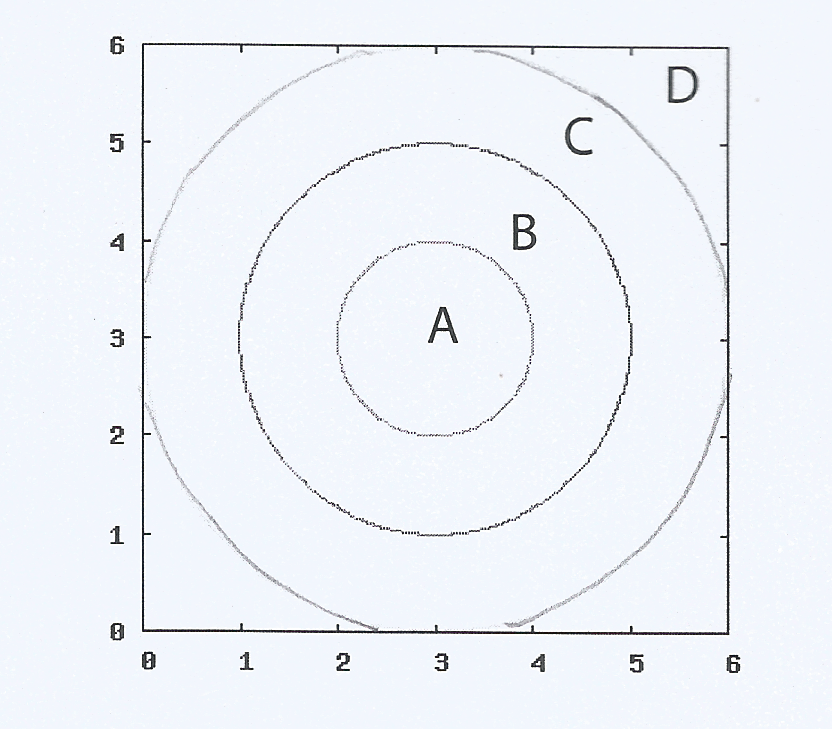
\includegraphics[scale=0.25]{diana.png}\\
Fig1: Diana que se usará en este trabajo.
\end{center}
\noindent En este proyecto analizaremos la práctica de tiro de un cadete en particular. Para este cadete, se dispone de 12 dianas  y en cada diana realizará 12 disparos. Las puntuaciones de cada disparo se ordenan en una matriz $A \in \mathbb{R}^{12\times 12}$ (\textit{matriz de puntuación de la semana 1}). Suponiendo que la matriz de puntuación de la semana $n$ esta dada por $A^n$ y la \textit{puntuación final de tiro de la semana $n$ }está dada por la norma de la matriz ($||A^n||_1\text{ o }||A^n||_\infty$), se desea hallar la puntuación final de tiro de la semana 10 usando ambas normas y concluir con qué norma sale más beneficiado el cadete.

\noindent La dificultad de este trabajo se centra en encontrar una expresión general para la potencia $n-$ésima de la matriz $A$, para esto vamos a usar la matriz de Jordan de $A$ ($J_A$) ya que se cumple $A^n=P^{-1}J^n_AP$, donde la potencia  $J^n_A$ es más fácil de hallar comparado a $A$.


\section{Fundamento Teórico}

\noindent Para dar con la descomposición canónica de Jordan de una matriz debemos introducir algunos conocimientos previos:

\begin{mydef}[Operadores Lineales Nilpotentes]
	El operador $T:V\to V$ es nilpotente si $T^{p} = 0$, para algún $p\in\mathbb{N}$. Además se dice que $k\in\mathbb{N}$ es el índice de nilpotencia de $T$ si $$T^{k-1}\neq 0 \ \wedge \ T^{k} = 0$$
\end{mydef}

\begin{mytheo}\label{theo_nilpotentes}  
    \noindent Sea $T:V\to V$, $V$ un $\mathbb{C}$ espacio vectorial, $\dim V = n$, $T$ nilpotente de índice $q$. Luego para $v\in V \ | \ T^{q-1}v\neq 0$, tenemos:
	\begin{enumerate}
		\item El conjunto $\{T^{q-1}v, T^{q-2}v,\ldots,Tv, v\}$ es L.I.
		\item S = $\left<\{T^{q-1}v, T^{q-2}v,\ldots,Tv, v\}\right>$ es invariante por $T$.
		\item Existe un subespacio $U$ de $V$, invariante por $T$ tal que:
		$$V = S\oplus U$$
	\end{enumerate}
\end{mytheo}

\begin{mycorol}
	Del teorema $(\ref{theo_nilpotentes})$
	\begin{align*}
		S &= \left<\{T^{q-1}v, T^{q-2}v,\ldots,Tv, v\}\right>\\
		&\Rightarrow\dim (S) = q\\			
	\end{align*}
%	Luego 
%	\begin{align*}
%		T(S) &= \left<\{T^{q-1}v, T^{q-2}v,\ldots,T^{2}v, Tv\}\right>\\
%		&\Rightarrow\dim T(S) = q-1\\\\
		%T^{2}(S) &= \left<\{T^{q-1}v, T^{q-2}v,\ldots,T^{3}v, T^{2}v\}\right>\\
		%&\Rightarrow\dim T^{2}(S) = q-2
%	\end{align*}
    Inductivamente 
	\begin{align*}
		T^{r}(S) &= \left<\{T^{q-1}v, T^{q-2}v,\ldots,T^{r+1}v, T^{r}v\}\right>\\
		&\Rightarrow\dim T^{r}(S) = q-r\\			
	\end{align*}
\end{mycorol}
\begin{mytheo}
\noindent Sea $T:V\rightarrow V$, dimV=n. Entonces existen $U, W \subset V$ invariantes por T tal que :
\begin{itemize}
    \item $V=U\oplus W$ 
    \item $T|_{U}:U\rightarrow U$ nilpotente  y $T|_{W}:W\rightarrow W$ inversible
\end{itemize}
\end{mytheo}
\noindent\textbf{NOTA:}
\noindent Como $T|_{U}:U\rightarrow U$ es nilpotente entonces existe $q\in\mathbb{N} \ | \  \left(T|_{U}\right)^{q}=0 $ y $(T|_{U})^{q-1}\neq 0$. Ahora hallamos un $v\neq0 \ | \ (T|_{U})^{q-1}v\neq 0$. Así definimos :\\
$B_{1}=\{(T|_{U})^{q-1}v, (T|_{U})^{q-2}v, ..., (T|_{U})v,v \}$ el cual es una base de U . Como W es invariante por T podemos definir $T|_{W}:W\rightarrow W$. Y volviendo a aplicar el teorema anterior $\exists \ U_{2}, W_{2} \subset W$ invariantes por T$\ | \  W=U_{2}\oplus W_{2}$, tal que \\
$T|_{U_{2}}: U_{2}\rightarrow U_{2}$ nilpotente y $T|_{W_{2}}:W_{2}\rightarrow W_{2}$ inversible.\\
Como $T|_{U_{2}}:U_{2}\rightarrow U_{2}$ nilpotente, $\exists \ q_{2} \in \mathbb{N} \ | \ (T|_{U_{2}})^{q_{2}}=0$ y $(T|_{U_{2}})^{q_{2}-1}\neq 0$, además  $q_{1}=q\geq q_{2}.$
Ahora hallando un $v_{2}\neq0$ tal que $ (T|_{U_{2}})^{q_{2}-1}v_{2}\neq 0$  de esto definimos \\
$B_{2}=\{(T|_{U_{2}})^{q_{2}-1}v_{2}, (T|_{U_{2}})^{q_{2}-2}v_{2}, ..., (T|_{U_{2}})v_{2},v_{2} \}$ el cual es una base para $U_{2}$. Luego de manera recursiva obtenemos: \\
$$V=U_{1}\oplus U_{2}\oplus U_{3}\oplus ... \oplus U_{k},$$ donde $U_{1}=U$. Luego $B=\displaystyle\bigcup\limits_{i-1}^{k}B_{i} $ es base de V y además \\
$$\left [T\right]_{B}=\begin{bmatrix}
	\left[T_{|U_{1}}\right]_{\beta_{1}}	&	O	&	\ldots	&	O\\
	O	&	\left[T_{|U_{2}}\right]_{\beta_{2}}	&	\ldots	&	O\\
	\vdots	&	\vdots	& \ddots	& \vdots\\
	O	&	O	&	\ldots	&	\left[T_{|U_{k}}\right]_{\beta_{k}}
\end{bmatrix}$$
 Donde 	$\left[T_{|U_{j}}\right]_{\beta_{j}}=\begin{bmatrix}
		0	&	1	&	0	&	0	&	\ldots	&	0\\
		0	&	0	&	1	&	0	&	\ldots	&	0\\
		0	&	0	&	0	&	1	&	\ldots	&	0\\
		\vdots	&	\vdots	&	\vdots	&	\vdots	&	\ddots	&	\vdots\\
		0	&	0	&	0	&	0	&	\ldots	&	1\\
		0	&	0	&	0	&	0	&	\ldots	&	0\\
	\end{bmatrix}_{q_{j}\times q_{j}}$

\vspace{0.7cm}



\begin{comment}
\begin{mynote}
Veamos como es la matriz de jordan para una matriz nilpotente.	Como $S = S_{1}$ es invariante por $T$, podemos definir el operador $T$ sobre $S_{1}$, es decir, $T:S_{1}\rightarrow S_{1}$ cuyo índice de nilpotencia es $q_{1} = q$.
Del teorema $(\ref{theo_nilpotentes})$, $\beta_{1} = \{T^{q-1}v, T^{q-2}v,\ldots,Tv, v\}$ es base de $S_{1}$.
Así 
\begin{align*}
	[T]_{\beta_{1}} &= 
	\left[
	\left[T\left(T^{q_{1}-1}v\right)\right], 
	\left[T\left(T^{q_{1}-2}v\right)\right],
	\left[T\left(T^{q_{1}-3}v\right)\right],
	\ldots,
	\left[T\left(Tv\right)\right],
	\left[T\left(v\right)\right]	
	\right]\\\\
	[T]_{\beta_{1}} &= 
	\begin{bmatrix}
		0	&	1	&	0	&	0	&	\ldots	&	0\\
		0	&	0	&	1	&	0	&	\ldots	&	0\\
		0	&	0	&	0	&	1	&	\ldots	&	0\\
		\vdots	&	\vdots	&	\vdots	&	\vdots	&	\ddots	&	\vdots\\
		0	&	0	&	0	&	0	&	\ldots	&	1\\
		0	&	0	&	0	&	0	&	\ldots	&	0\\
	\end{bmatrix} = [T_{|S1}]_{\beta_{1}}
\end{align*}
Además como $U = U_{1}$ invariante por $T$, podemos definir $T$ sobre $U_{1}$, $T: U_{1}\rightarrow U_{1}$, y volver a aplicar el \textit{teorema}$(\ref{theo_nilpotentes})$, es decir existe $S_{2}$ y $U_{2}$ subespacios de $U_{1}$, invariantes por $T$/
$$U_{1} = S_{2}\oplus U_{2}$$
Repitiendo lo anterior pero con $S = S_{2},\exists u\in V/T^{q_{2}-1}u\neq 0$, donde $q_{2}$ es el índice de nilpotencia de $T_{|S} = T:S\rightarrow S$, asi:
\begin{align*}
	\beta_{2} &= \left\{T^{q_{2}-1}u, T^{q_{2}-2}u,\ldots,Tu, u\right\}
\end{align*}
$$[T]_{\beta_{2}} = 
\begin{bmatrix}
	0	&	1	&	0	&	0	&	\ldots	&	0\\
	0	&	0	&	1	&	0	&	\ldots	&	0\\
	0	&	0	&	0	&	1	&	\ldots	&	0\\
	\vdots	&	\vdots	&	\vdots	&	\vdots	&	\ddots	&	\vdots\\
	0	&	0	&	0	&	0	&	\ldots	&	1\\
	0	&	0	&	0	&	0	&	\ldots	&	0\\
\end{bmatrix} = [T_{|S2}]_{\beta_{2}}$$
$$$$
Podemos continuar descomponiendo los $U_{k}$, por el teorema anterior, hasta obtener:
$$V = S_{1}\oplus S_{2}\oplus \ldots \oplus S_{k}$$
De esto $\beta = \bigcup_{i=1}^{k}\beta_{i}$ es base de $V$, donde $\beta_{i}$ es base de $S_{i}$.
Además
$$\begin{bmatrix}
	\left[T_{|S_{1}}\right]_{\beta_{1}}	&	O	&	\ldots	&	O\\
	O	&	\left[T_{|S_{2}}\right]_{\beta_{2}}	&	\ldots	&	O\\
	\vdots	&	\vdots	& \ddots	& \vdots\\
	O	&	O	&	\ldots	&	\left[T_{|S_{k}}\right]_{\beta_{k}}
\end{bmatrix}$$

Note que el bloque $\left[T_{|S_{k}}\right]_{\beta_{k}}$ es más grande (o igual) que el bloque $\left[T_{|S_{m}}\right]_{\beta_{m}}$, para $k > m$, pues $q_{k}\geq q_{m}$.
De esta forma obtendríamos la forma canónica de una matriz nilpotente.
\end{mynote}
\end{comment}


\begin{mytheo}[Forma Canónica de Jordan]
	Sea $V$ un $\mathbb{C}$-espacio vectorial, $\dim V = n$, $T:V\rightarrow V$ un operador lineal y $\lambda_{1},\lambda_{2},\ldots,\lambda_{k}\in \wedge (T)$ y $n_{1}, n_{2},\ldots , n_{k}$ las multiplicidades algebraicas de los valores propios (respectivamente), entonces:

Existen subespacios $V_{1}, V_{2},\ldots, V_{k}$ invariantes por $T\;\left(T(V_{i})\subseteq V_{i}\right) |$
\begin{enumerate}
	\item	$V = V_{1}\oplus V_{2}\oplus\ldots\oplus V_{k}$
	\item $\dim V_{i} = n_{i},\quad i=1-k$
	\item El operador $T-\lambda_{i}I:V_{i}\rightarrow V_{i}$ es nilpotente, $i=1-k$. (Aquí se aplica la propiedad ya antes mencionada para un operador nilpotente)
	
	
\end{enumerate}
\end{mytheo}
\noindent Ahora introduciremos a algunos métodos numéricos que nos permiten calcular los valores y vectores  propios de una matriz, los cuales son necesarios para construir la forma canónica de Jordan de una matriz:\\
\subsection{Cálculo del Valor propio y Vector propio}
\noindent Dada una matriz $A\in \mathbb{R}^{n\times n}$, este método calcula el mayor valor propio de $A$ y el vector propio asociado a este valor propio, mediante iteraciones.
Es decir, dada la siguiente relación de recurrencia :\begin{equation}
    q^{(k+1)} = \frac{1}{\phi_{k}}Aq^{(k)},\quad donde\;\phi_{k} = \Vert Aq^{(k)}\Vert    
\end{equation} e inicializando con algún vector $q^{(0)}$, al realizar las iteraciones la sucesión converge al autovector asociado al mayor valor propio.


\subsection{Convergencia del Método Potencia}%(Caso particular y caso general)}
\begin{itemize}
	%\item Caso particular\\Si cada $\lambda\in\wedge (A)$ tiene mutiplicidad $1$, luego podemos ordenarlos(los valores propios), de la siguiente forma:
	%$$\vert \lambda_{1}\vert >\vert\lambda_{2}\vert >\ldots >\vert\lambda_{n}\vert$$
	
	%Ahora sea $M=\{v_{1}, v_{2},\ldots, v_{n}\}$ los vectores propios asociados a los valores propios(respectivamente, $Av_{i} = \lambda_{i}v_{i}$). Así M es una base de $\mathbb{R}^{n\times 1}$. Por lo tanto para $q^{(0)}\in\mathbb{R}^{n\times 1}, q^{(0)}\in M$, tenemos:
	%$$q^{(0)} = \sum_{k=1}^{n}c_{k}v_{k}$$
	

%Asi podemos definir la siguiente sucesión %(la cual probaremos que converge a $x_{1}$)
%$$q^{(k+1)} = \frac{1}{\phi_{k}}Aq^{(k)},\quad donde\;\phi_{k} = \Vert Aq^{(k)}\Vert$$ la cual converge al vector propio del mayor valor propio.
\begin{comment}


\begin{align*}
	q^{(k+1)} &= \frac{1}{\phi_{k}}A\left(\frac{1}{\phi_{k-1}}Aq^{(k-1)}\right)\\
		&= \frac{1}{\phi_{k}\phi_{k-1}}A^{2}q^{(k-1)}\\
		&= \frac{1}{\phi_{k}\phi_{k-1}\phi_{k-2}}A^{3}q^{(k-2)}\\
		&\vdots\\
		&= \frac{1}{\phi_{k}\phi_{k-1}\ldots\phi_{0}}A^{k+1}q{(0)}\\\\
	q^{(k+1)} &= \left(\prod_{i=0}^{k}\phi_{i}^{-1}\right)A^{k+1}q^{(0)}\\
		&= \phi A^{k+1}\left(\ds\sum_{j=1}{n}c_{j}x_{j}\right),\quad\phi = \left(\prod_{i=0}^{k}\phi_{i}^{-1}\right)\\
		&= \phi \ds\sum_{j=1}{n}c_{j}A^{k+1}x_{j}\\
		&= \phi \ds\sum_{j=1}{n}c_{j}\lambda_{j}^{k+1}x_{j}\\
		&= \phi\lambda_{1}^{k+1}\left(c_{1}x_{1} + \ds\sum_{j=2}^{n}c_{j}\left(\frac{\lambda_{j}}{\lambda_{1}}\right)^{k+1}x_{j}\right)
\end{align*}


Como $\left\vert\frac{\lambda_{j}}{\lambda_{1}}\right\vert < 1,\quad j=2-n$, entonces:
$$\lim_{k\rightarrow\infty}q^{(k+1)} = \left(\lim_{k\rightarrow\infty}\prod_{i=0}^{k}\lambda_{j}^{k+1}\right)(c_{1}x_{1}+0)$$
$$\therefore\quad\lim_{k\rightarrow\infty}q{(k+1)} = c_{1}ax_{1},\quad donde\quad a = \left(\lim_{k\rightarrow\infty}\prod_{i=0}^{k}\lambda_{j}^{k+1}\right)$$



\\Ahora vamos a construir una sucesión que converja al valor propio $\lambda_{1}$.
\begin{equation}\label{eigenvalue_iter}
u^{(k+1)} = \frac{1}{\phi_{k}}\frac{(Aq^{(k)})_{j}}{q^{(k)}_{j}}
\end{equation}
donde $(Aq^{(k)})_{j}$ es el j-ésimo elemento de $Aq^{(k)}$ y $q^{(k)}_{j}$ es el j-ésimo elemento de $q^{(k)}$
\end{comment}
\begin{comment}


Vamos a denotar $x_{ij}$ al j-ésimo elemento de $x_{i}$. Como 
\begin{align*}
	Aq^{(k)} &= \phi_{k}q^{(k+1)}\\
	\Rightarrow	Aq^{(k)}_{j} &= \phi_{k}q^{(k+1)}_{j}\\
	\Rightarrow	u^{(k+1)} &= \frac{1}{\phi_{k}}\frac{\phi_{k}(q^{(k+1)})_{j}}{q^{(k)}_{j}} = \frac{q_{j}^{(k+1)}}{q_{j}^{(k)}}\\
\end{align*}

Como 
$$ q{(m)} = \phi\lambda_{1}^{m+1}\left(c_{1}x_{1} + \sum_{i=2}^{n}c_{i}\left(\frac{\lambda_{j}}{\lambda_{1}}\right)^{m+1}x_{i}\right),\quad m\in\mathbb{N}$$

En $(\ref{eigenvalue_iter})$
\begin{align*}
	u^{(k+1)} &= \frac{\phi\lambda_{1}^{k+1}\left(c_{1}x_{1j} + \ds\sum_{i=2}^{n}c_{i}\left(\frac{\lambda_{j}}{\lambda_{1}}\right)^{k+1}x_{ij}\right)}{\phi\lambda_{1}^{k}\left(c_{1}x_{1j} + \ds\sum_{i=2}^{n}c_{i}\left(\frac{\lambda_{j}}{\lambda_{1}}\right)^{k}x_{ij}\right)}\\
		&= \lambda_{1}\left[\frac{c_{1}x_{1j} + \ds\sum_{i=2}^{n}c_{i}\left(\frac{\lambda_{j}}{\lambda_{1}}\right)^{k+1}x_{ij}}{c_{1}x_{1j} + \ds\sum_{i=2}^{n}c_{i}\left(\frac{\lambda_{j}}{\lambda_{1}}\right)^{k}x_{ij}}\right]\\
	\Rightarrow	\lim_{k\rightarrow\infty}u^{k+1} &= \lambda_{1}\lim_{k\rightarrow\infty}	\frac{c_{1}x_{1j} + \ds\sum_{i=2}^{n}c_{i}\left(\frac{\lambda_{j}}{\lambda_{1}}\right)^{k+1}x_{ij}}{c_{1}x_{1j} + \ds\sum_{i=2}^{n}c_{i}\left(\frac{\lambda_{j}}{\lambda_{1}}\right)^{k}x_{ij}} = \lambda_{1}\left(\frac{c_{1}x_{1}}{c_{1}x_{1}}\right) = \lambda_{1}
\end{align*}
\end{comment}

    

\item Caso general:\\
Sea $\wedge(A)=\{\lambda_{1},\lambda_{2},\ldots ,\lambda_{k}\}$ y $m_{1},m_{2}, \ldots , m_{k}\in\mathbb{N}$ multiplicidades geométricas de $\lambda_{1},\lambda_{2},\ldots ,\lambda_{k}$ respectivamente (no necesariamente $V=V_{1}\oplus V_{2}\oplus V_{3}\oplus\ldots\oplus V_{k}, V_{i}$ espacio propio de $\lambda_{i}$).
	
Sin pérdida de la generalidad, sea:
$$\vert\lambda_{1}\vert > \vert\lambda_{2}\vert > \vert\lambda_{3}\vert > \ldots>\vert\lambda_{k}\vert$$
	
Ahora sea $q^{(0)}\in\left<\bigcup_{i=1}^{k}V_{i}\right>$
$$\Rightarrow\quad q^{(0)} = \sum_{i=1}^{m_{1}}c_{i}^{(1)}v_{i}^{(1)} + \sum_{r=1}^{k}\sum_{j=1}^{m_{r}}c_{j}^{(r)}v_{j}^{(r)}$$
donde $v_{j}^{(i)}$: vector j-ésimo del espacio propio $v_{i}$.



En este caso la sucesión $$q^{(k+1)}=\frac{1}{\phi_{k}}Aq^{(k)}$$ converge a un múltiplo del vector propio asociado a mayor valor propio.\\
\end{itemize}

Ahora, se construye la siguiente sucesión que converge al valor propio $\lambda_{1}$.
\begin{equation}\label{eigenvalue_iter}
u^{(k+1)} = \frac{1}{\phi_{k}}\frac{(Aq^{(k)})_{j}}{q^{(k)}_{j}}
\end{equation}
donde $(Aq^{(k)})_{j}$ es el j-ésimo elemento de $Aq^{(k)}$ y $q^{(k)}_{j}$ es el j-ésimo elemento de $q^{(k)}.$\\
Así las ecuaciones (1) y (2) nos servirán para hallar el vector propio y su respectivo valor propio siendo este el máximo.


\subsection{Deflacción}
\noindent Luego que se ha obtenido $\lambda_{1}$ el autovalor máximo y $x_{1}$ su autovector propio asociado mediante el método de la potencia de una matriz $A^{n\times n}$, utilizaremos la deflacción para hallar una matriz mas simple que tenga los mismos autovalores que A sin contar el autovalor ya calculado es decir el $\lambda_{1}$, como esta matriz tendrá los mismos autovalores de A ( sin el $\lambda_{1}$), podemos aplicarle el método de la potencia para hallar el siguiente autovalor ($\lambda_{2}$) y luego volver a aplicar la deflación para hallar una matriz más simple que contenga los mismos autovalores de A pero sin $\lambda_{1}$ y $\lambda_{2}$, con el método de la potencia obtenemos otro autovalor $\lambda_{3}$ y así recursivamente encontramos todos los autovalores de A.
Esto sigue el siguiente esquema:\\
Sea el $x$ un autovector de A y $\lambda $ su correspondiente autovalor. Y sea U una matriz $n\times(n-1)$ tal que (x,U) sea unitario. ya que Ax=$\lambda$x y $A(x,A)=(Ax,AU)$, tenemos$$(X,U)^{H}A(x,U)=\left(\begin{array}{c}
    x^{H} \\
     U^{H} 
\end{array}\right)\left((\lambda x,AU)\right)$$ $$=\newline \left(\begin{array}{cc}
   \lambda x^{H}x  &  x^{H}AU\\
   \lambda U^{H}x  & U^{H}AU
\end{array}\right)$$
Ahora $x^{H}x=1$  y x es ortogonal a las columnas de U, es decir, $U^{H}X=0$. Luego:\\
$$(x,U)^{H}A(x,U)=\left(\begin{array}{cc}
  \lambda   &  h^{H}\\
    0 & C
\end{array}\right)...(*)$$ Donde $C=U^{H}AU$ es de orden  $(n-1)\times (n-1)$ y $h^{H}=x^{H}AU$. Así la matriz(*) tiene como autovalores a $\lambda$ y a los autovalores de C y como esta matriz es semejante a A tienen los mismo autovalores por eso solo implicaría hallar los autovalores de la matriz C.\\
Ahora, para determinar U usamos las transformaciones de Householder.\\

\noindent\textbf{Propiedad}\\
\noindent Si x $\in\mathbb{R}^n, \ x_{1}$ su primera componente, $x\neq 0,\ \sigma=sign(x_{1})\|x\|_{2}$ donde $sign(0)=+1$, y si $w=x+\sigma e^{(1)} \ y \ \theta=\frac{1}{2}{\|w\|}^{2}_{2}$, \ luego $$W=I-\frac{1}{\theta}ww^{H}$$ es la transformación de Householder con $Wx=-\sigma e^{(1)}$.\\
Siendo $\lambda$ el autovalor hallado de A y x su respectivo autovector construiremos la transformación T usando la propiedad de modo que:  $$Tx=-sign(x_{1})\|x\|_{2}e^{(1)}=-sign(x_{1})e^{(1)}$$ asumiendo además $\|x\|_{2}=1$, luego:\\
$$T^{2}=x=-sign(x_{1})Te^{(1)}$$ya que T es unitaria. De aquí se obtiene $Te^{(1)}=-sign(x_{1})x$. De esto, la primera columna de T es el autovector $-sign(x_{1})x$. Por lo tanto $T=(-sign(x_{1})x,U)$ donde U resulta ser unitario de orden $n\times(n-1)$, de esta forma encontramos U. \\

\noindent Con el método de la potencia y la deflacción podremos hallar todos los autovalores propios de nuestra matriz, así obtenemos la forma canónica de jordan $J$, $A=PJP^{-1}$, donde P es la matriz de cambio de base (de una base B' de V a la base formada por los $B_{i}$ como se mostró anteriormente).\\

%\noindent Los siguientes dos métodos los utilizaremos también para calcular los autovalores de A, a fin de comparar los resultados finales para la resolución del problema.

%\section{Método QR}
%\section{Doble QR}
\end{multicols}{2}
\newpage
\section{Análisis}
\begin{enumerate}
	\item \label{item1} Construye una matriz que recoja los datos obtenidos en la prueba de tiro por el Caballero Cadete en estudio.
		Matriz de puntuaciones semana 1


$$\begin{bmatrix}
	1	&	0	&	0	&	0	&	\ldots   &	0	&	0	&	0	&	0\\
	0	&	s	&	0	&	0	&   \ldots   &	0	&	0	&	0	&	0\\
	1	&	1	&	s	&	0	&	\ldots   &	0	&	0	&	0	&	0\\
	0	&	0	&	0	&	1	&	\ldots   &	0	&	0	&	0	&	0\\
	0	&	0	&	0	&	0	&	\ldots 	 &	0	&	0	&	0	&	0\\
	0	&	0	&	0	&	0	&	\ldots	&	0	&	0	&	0	&	0\\
	0	&	0	&	0	&	0	&	\ldots	&	0	&	0	&	0	&	0\\
	0	&	0	&	0	&	0	&	\ldots	&	s	&	0	&	0	&	0\\
	0	&	0	&	0	&	0	&	\ldots	&	1	&	s	&	0	&	0\\
	0	&	0	&	0	&	0	&	\ldots	&	0	&	1	&	s	&	0\\
	0	&	0	&	0	&	0	&	\ldots	&	0	&	0	&	1	&	s\\
	0	&	0	&	0	&	0	&	\ldots	&	0	&	0	&	0	&	1
\end{bmatrix}$$
	
	\item Calcule una expresión general para la potencia k-ésima de la matriz de \ref{item1}
	$$	
	\begin{bmatrix}
	-\frac{-s+1}{s-1}	&	0	&	0	&	0	&	\ldots	&	0	&	0	&	0	&	0\\
	0	&	s^{k}	&	0	&	0	&	\ldots	&	0	&	0	&	0	&	0\\
	\frac{s^{k}}{s-1} - \frac{1}{s-1}	&	ks^{(k - 1)}	&	s^{k}	&	0	&	\ldots	&	0	&	0	&	0	&	0\\
	0	&	0	&	0	&	1	&	\ldots	&	0	&	0	&	0	&	0\\
	0	&	0	&	0	&	0	&	\ldots	&	0	&	0	&	0	&	0\\
	0	&	0	&	0	&	0	&	\ldots	&	0	&	0	&	0	&	0\\
	0	&	0	&	0	&	0	&	\ldots	&	0	&	0	&	0	&	0\\
	0	&	0	&	0	&	0	&	\ldots	&	ks	&	\frac{ks^{2}(k - 1)}{2}	&	\frac{ks^{3}(k - 2)(k - 1)}{6}	&	\frac{ks^{4}(k - 3)(k - 2)(k - 1)}{24}\\
	0	&	0	&	0	&	0	&	\ldots	&	1	&	ks	&	\frac{ks^{2}(k - 1)}{2}	&	\frac{s^{3}(k - 2)(k - 1)}{6}\\
	0	&	0	&	0	&	0	&	\ldots	&	0	&	1	&	ks	&	\frac{ks^{2}(k - 1)}{2}\\
	0	&	0	&	0	&	0	&	\ldots	&	0	&	0	&	1	&	ks\\
	0	&	0	&	0	&	0	&	\ldots	&	0	&	0	&	0	&	1	
	\end{bmatrix}		
	$$
	
	\item Suponiendo que la matriz de puntuación del Caballero Cadete en tiro la semana k se obtiene con la potencia k de la matriz obtenida en la primera práctica, calcule la matriz de puntuaciones obtenidas por dicho Caballero Cadete en la semana 10 de curso, sabiendo que la bonificación de diana en esa semana es 5 puntos.
	
	Matriz de puntuaciones de la semana  10.
	$$
	A^{10}=
	\begin{bmatrix}
1.0	&	0	&	0	&	0	&	\ldots	&	0	&	0	&	0	&	0\\
0	&	9765625.0	&	0	&	0	&	\ldots	&	0	&	0	&	0	&	0\\
2441406.0	&	19531250.0	&	9765625.0	&	0	&	\ldots	&	0	&	0	&	0	&	0\\
0	&	0	&	0	&	1.0	&	\ldots	&	0	&	0	&	0	&	0\\
0	&	0	&	0	&	0	&	\ldots	&	0	&	0	&	0	&	0\\
0	&	0	&	0	&	0	&	\ldots	&	0	&	0	&	0	&	0\\
0	&	0	&	0	&	0	&	\ldots	&	0	&	0	&	0	&	0\\
0	&	0	&	0	&	0	&	\ldots	&	50.0	&	1125.0	&	15000.0	&	131250.0\\
0	&	0	&	0	&	0	&	\ldots	&	1.0	&	50.0	&	1125.0	&	15000.0\\
0	&	0	&	0	&	0	&	\ldots	&	0	&	1.0	&	50.0	&	1125.0\\
0	&	0	&	0	&	0	&	\ldots	&	0	&	0	&	1.0	&	50.0\\
0	&	0	&	0	&	0	&	\ldots	&	0	&	0	&	0	&	1.0
\end{bmatrix}	
	$$    
	
	
	\item La puntuación final en tiro de una semana se obtiene calculando la norma de una matriz. Considerando que las normas utilizadas son $\Vert A\Vert_{\infty}$ y $\Vert A\Vert_{1}$ . Calcule la puntación final que obtendría el Caballero Cadete en estudio en la semana 10 del curso (bonificación diana 5 puntos) si se aplica cada una de las normas anteriores. ¿ Con qué norma saldría beneficiado ?
		\begin{itemize}
			\item $\Vert A^{10}\Vert_{\infty} = 31738281.0000000$
			\item $\Vert A^{10}\Vert_{1} = 29296875.0000000$
		\end{itemize}
		$\therefore$ EL Caballero Cadete se verá beneficiado si su puntuación se calcula con la norma del máximo $(\Vert .\Vert_{\infty})$
\end{enumerate}


\newpage
\begin{center}
 -----------------------------------------------------------------------------------
\end{center}
\begin{multicols}{2}
\begin{list}{}{\setlength{\topsep}{0mm}\setlength{\itemsep}{0mm}%
\setlength{\parsep}{0mm}\setlength{\leftmargin}{4mm}}
%
%------------------------------------- References --------------------
\small
\item[1.] Azmy S Ackleh. \textit{Classical and modern numerical analysis}, Chapman \& Hall/CRC (2010).
\item[2.] David Kincaid, Ward Cheney. \textit{Numerical Analysis Mathematics of Scientific Computing}, 3rd edition (2002).
\item[3.] Claus Fuhrer, Jan Erik Solem, Olivier Verdier. \textit{Scientific Computing with Python 3}, 2nd edition(2017).
%---------------------------------------------------------------------
%
\end{list}
\end{multicols}


\end{document}
